% !TeX program = lualatex

% Per https://github.com/matze/mthemem, Fira fonts needs to be installed in the system.
% If fonts do not metter, just use pdflatex instead of lualatex (and also remove luatex85 depnedency below)

\documentclass{beamer}
\usetheme{metropolis}

\usepackage{luatex85}
\usepackage{multimedia}
\usepackage{graphicx}
\usepackage{multicol}
\usepackage{qrcode}

\usepackage{mathtools}
\mathtoolsset{showonlyrefs}

\usepackage[absolute,overlay]{textpos}
\setlength{\TPHorizModule}{\paperwidth}
\setlength{\TPVertModule}{\paperheight}

% https://tex.stackexchange.com/a/43005
\newlength{\currentparskip} 
\newenvironment{minipageparskip}[1]{\setlength{\currentparskip}{\parskip}\begin{minipage}{#1}\setlength{\parskip}{\currentparskip}}{\end{minipage}}

% END OF CONFIGURATION

\title{MAE 259B Group 2 Progress Report}
\date{\url{https://github.com/kmxz/mae259b-project}}
\author{Siyuan Chen, Xiangzhou Kong, Long Chen}

\begin{document}
    \maketitle
    \begin{frame}{What we did - Starting point}
        \textbf{Start from the homework code}\\
	    Adapted from the MATLAB sample code, translated into Python, with minor changes and optimizations
        
        \textbf{Build utilities}\\
        Command line interface, 3D visualization tool, code snapshot tool, etc.
        
        \begin{center}
        	 \movie[width=4.0073cm,height=3.3927cm,showcontrols,poster,loop]{(Video: hw-render)}{res/hw-render.mp4}
        	 \hspace{2cm}
        	 \movie[width=4.0073cm,height=3.3927cm,showcontrols,poster,loop]{(Video: hw-nodes)}{res/hw-nodes.mp4} 
        \end{center}
    \end{frame}
    \begin{frame}{What we did - Performance optimization}
    	Profiling shows $90\%$ of time is spent on calculating $F$ and $J$
    	
    	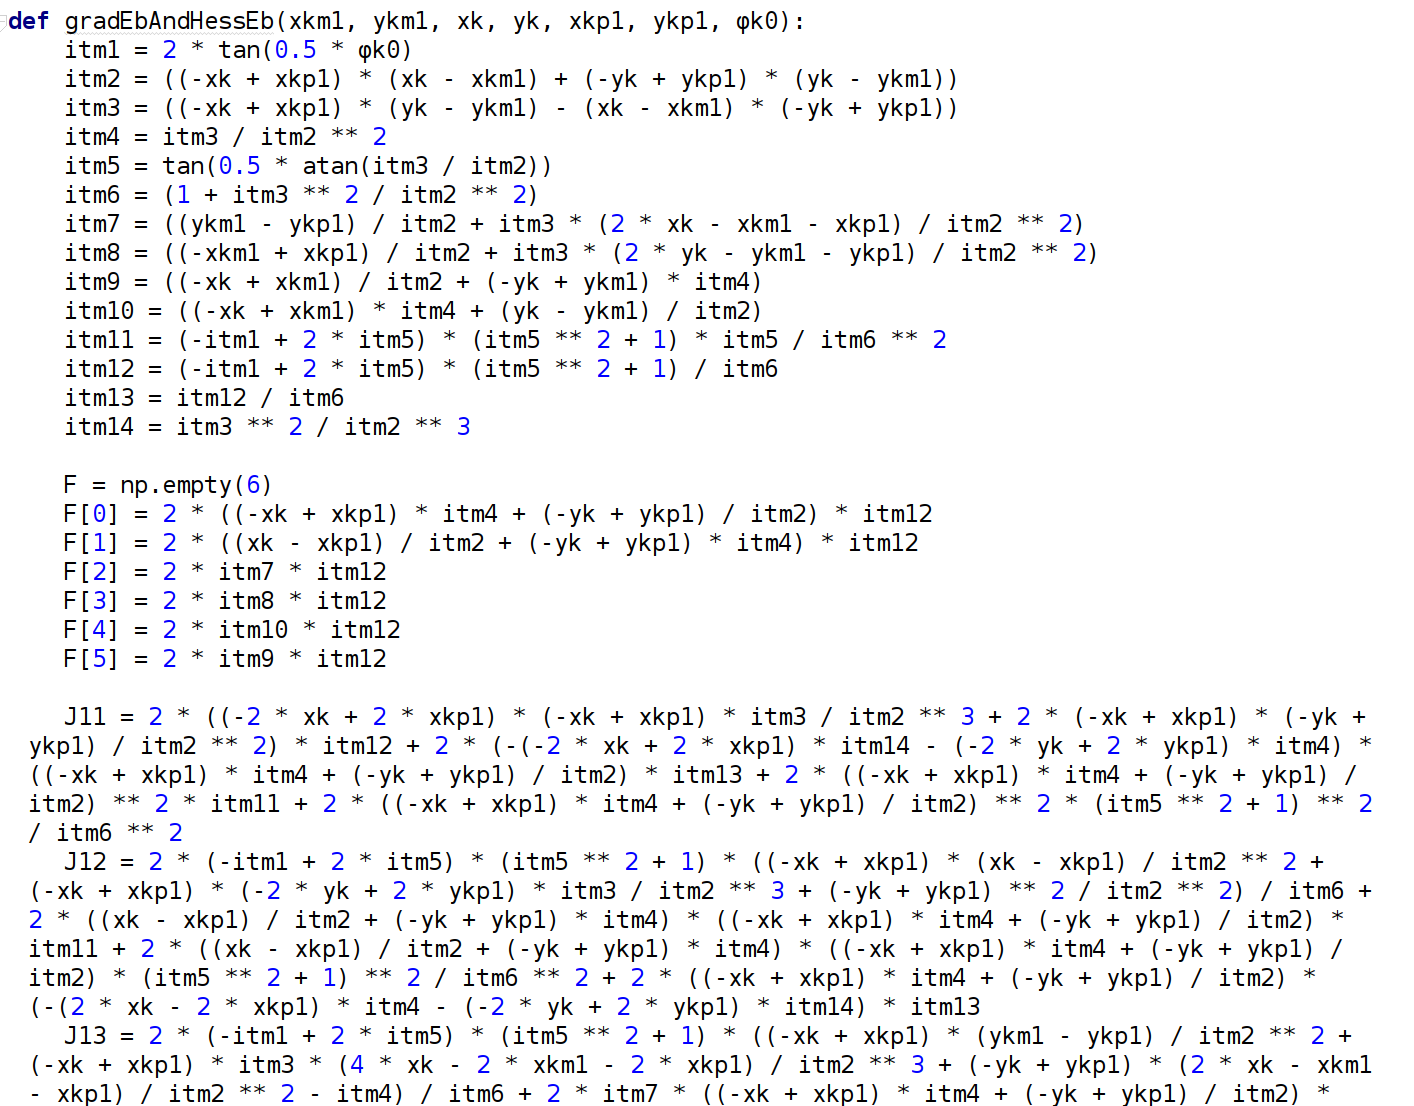
\includegraphics[width=0.9\textwidth]{res/getFb.png}
    	\begin{textblock}{0.3}[1,0](1,0.25)
		    \begin{center}
		    	\Large $30.6\,\mathrm s$\\$\Downarrow$\\$7.6\,\mathrm s$\\\bf 4x faster
		    \end{center}
    	\end{textblock}
	\end{frame}
	\begin{frame}{What we did - Natural curvature}
		\begin{minipageparskip}{0.5\textwidth}
			When calculating bending energy, replace $\frac12EI(\phi_k)^2$ with $\frac12EI(\phi_k - \phi_{k0})^2$
			
			The formulas for calculating $F$ and $J$ need to be changed (do differentiation again)
			
			\footnotesize
			To verify the result:
			\begin{itemize}
				\item Expect same result as previous code when $\phi_0$ = 0
				\item Expect a straight beam to recover natural curvature when no external force applied
			\end{itemize}
		\end{minipageparskip}%
		\hspace{0.05\textwidth}%
		\begin{minipageparskip}{0.45\textwidth}
			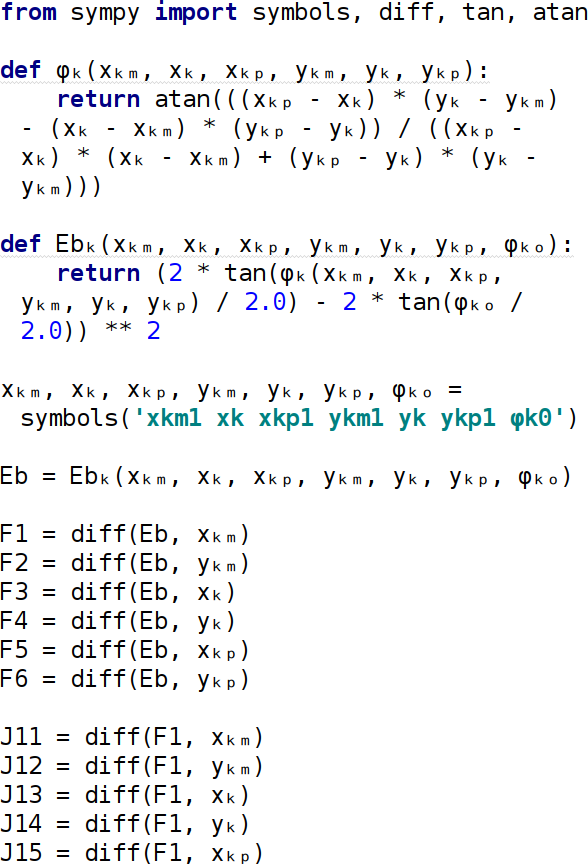
\includegraphics[width=\textwidth]{res/diff.png}
		\end{minipageparskip}
	\end{frame}
	\begin{frame}{What we did - Circular structure}
		\small
		Instead of $nv - 1$ edges, we have $nv$ edges.\\
		For bending, instead of $nv - 2$ components, we have $nv$ components.\\
		For stretching, instead of $nv - 1$ components, we have $nv$ components.
		
		When compositing the Jacobians, new components added to connect two ends together:
		
		\begin{center}
			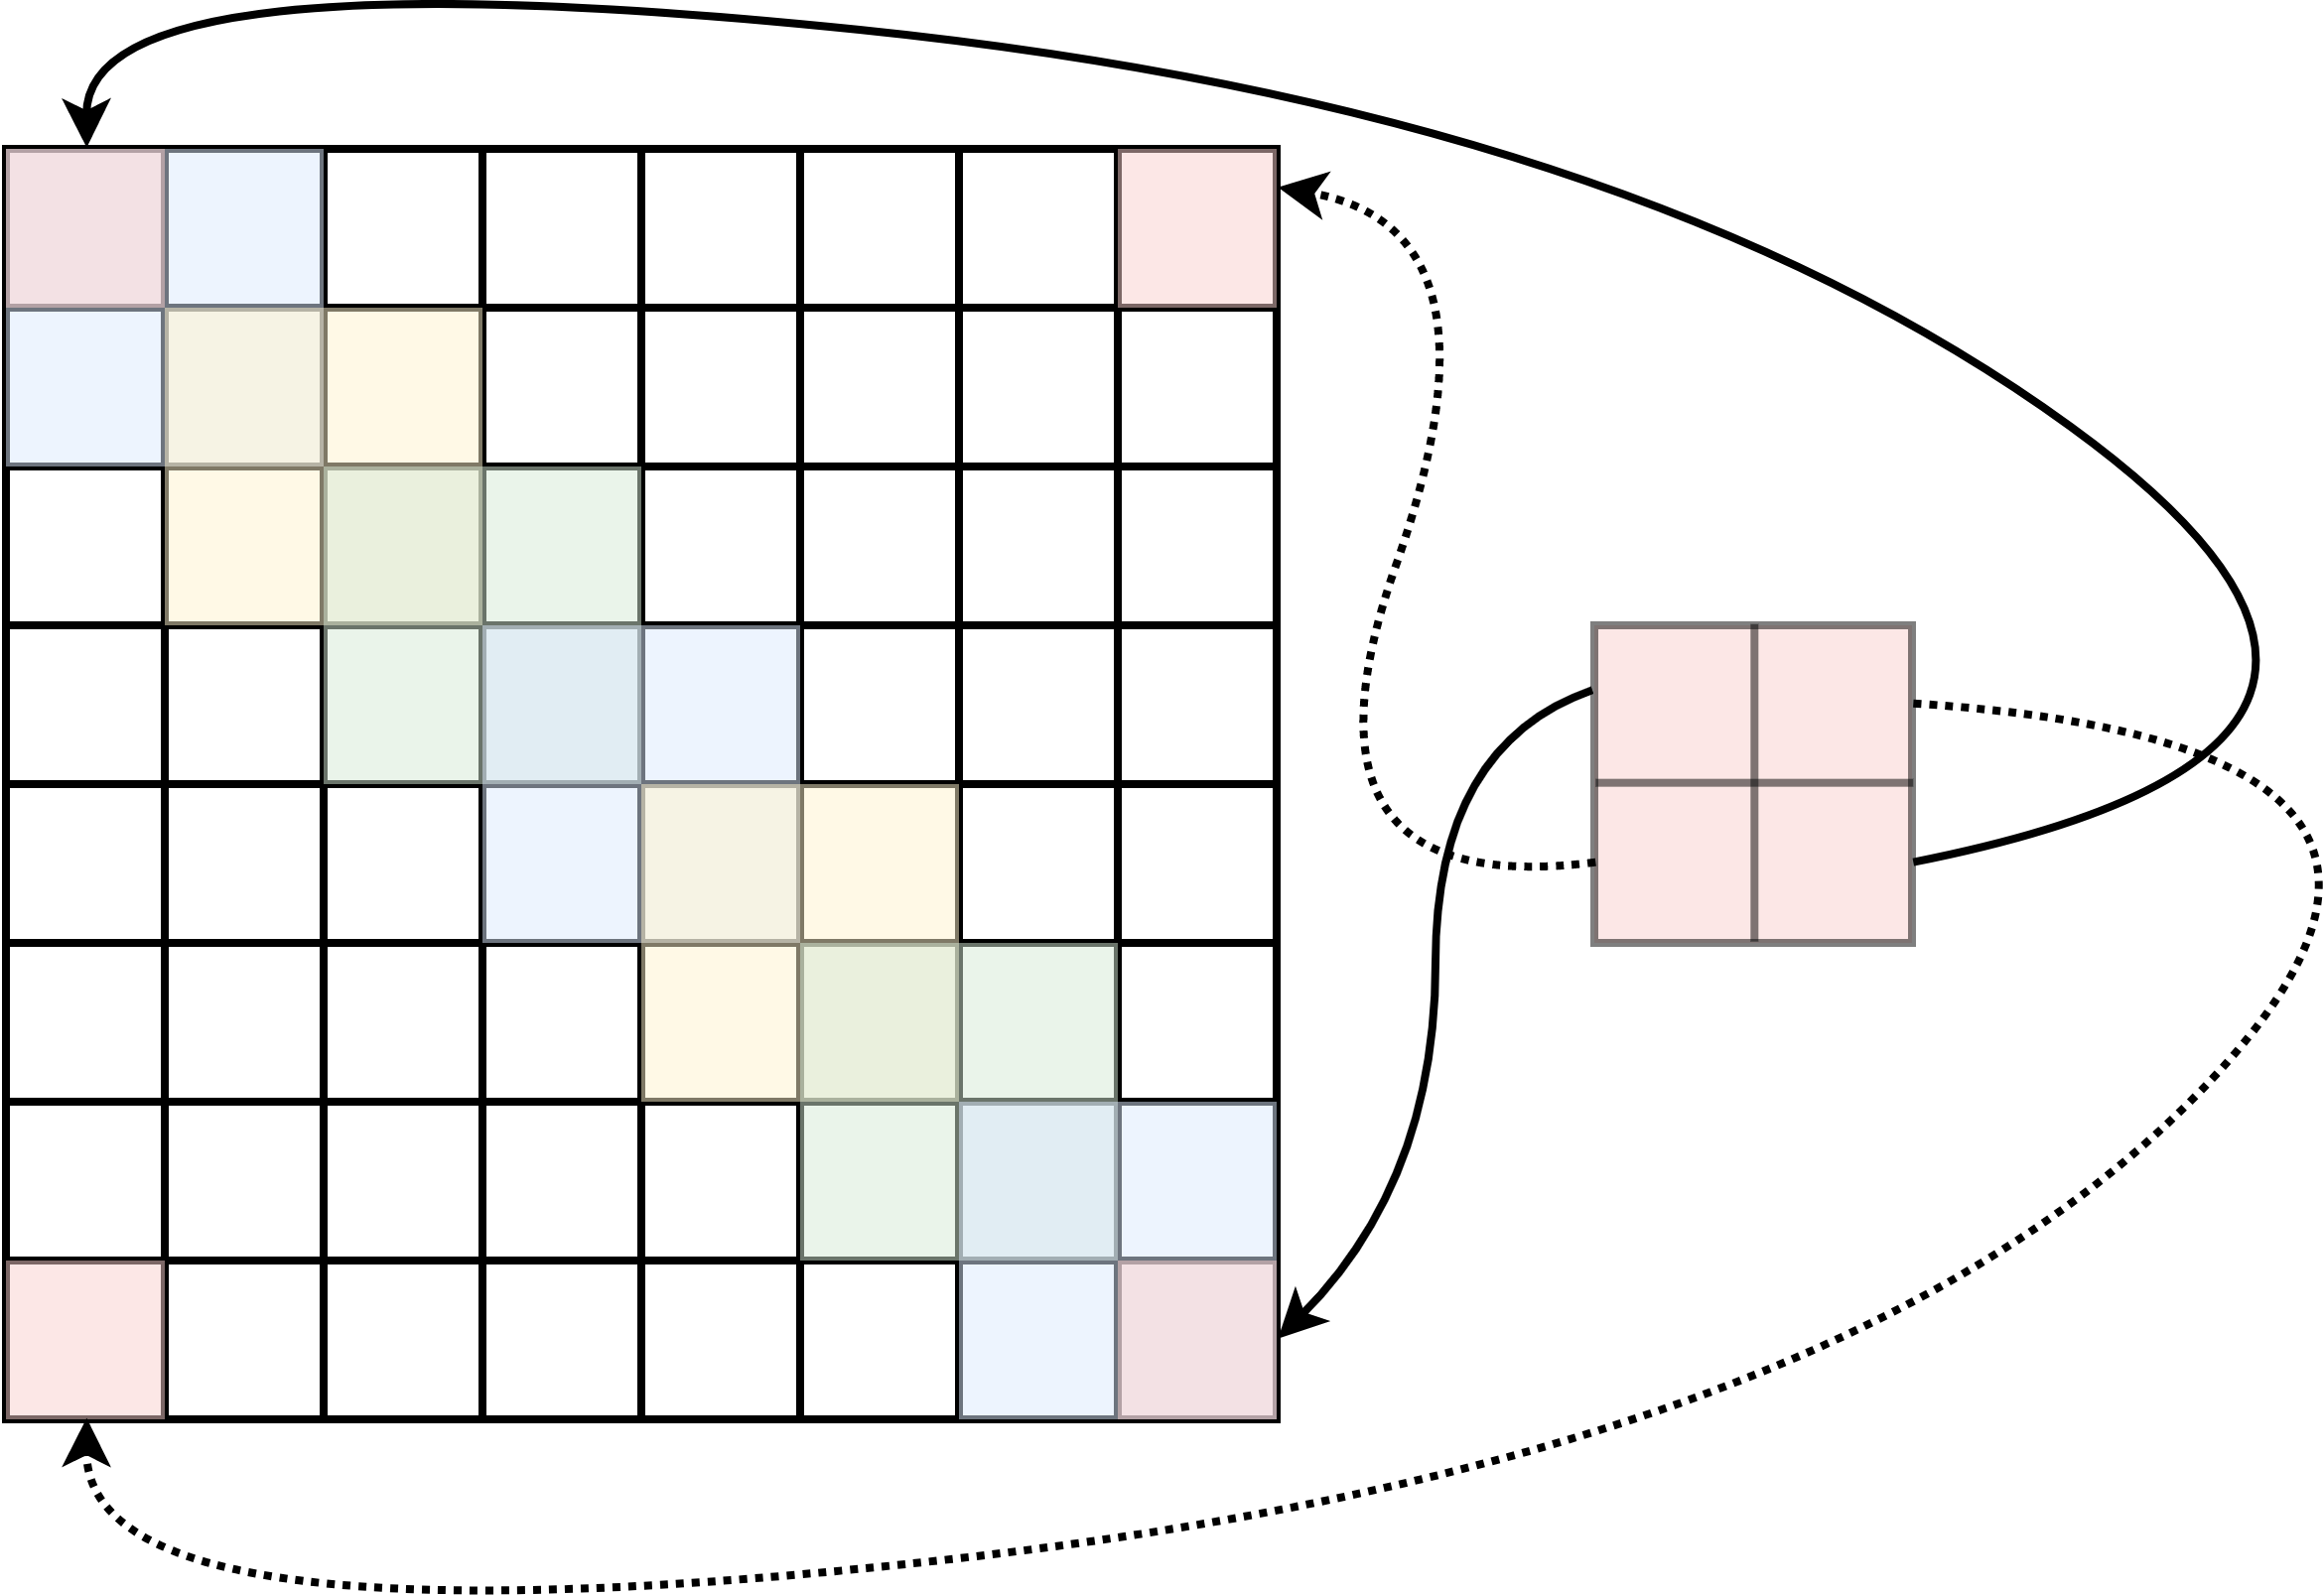
\includegraphics[width=0.6\textwidth]{res/composition.png}
		\end{center}
	\end{frame}
	\begin{frame}{What we did - Circular structure}
		Verify our code by running the ``hanging circle''
		
		\begin{tabular}{ccc}
			$Y = 10^6\,\mathrm{Pa}$ & $Y = 10^7\,\mathrm{Pa}$ & $Y = 10^8\,\mathrm{Pa}$\\
			\movie[width=3.09cm,height=3.11cm,showcontrols,poster,loop]{(Video: 1e6)}{res/1e6.mp4} & 
			\movie[width=3.09cm,height=3.11cm,showcontrols,poster,loop]{(Video: 1e7)}{res/1e7.mp4} & 
			\movie[width=3.09cm,height=3.11cm,showcontrols,poster,loop]{(Video: 1e8)}{res/1e8.mp4}
		\end{tabular}
	\end{frame}
	\begin{frame}{What we did - Inflation pressure}
		\begin{center}
			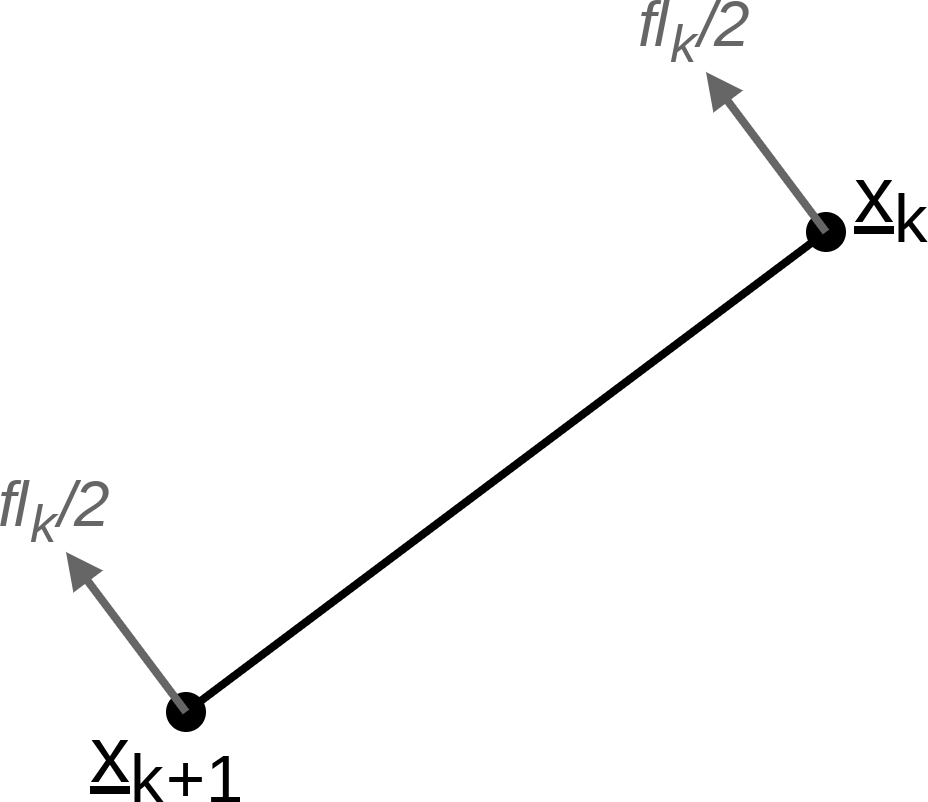
\includegraphics[width=0.4\textwidth]{res/inflation.png}
		\end{center}
	
		With $\underline x_k$ and $\underline x_{k+1}$, we can easily calculate force exerted on those two points. 
		
		As force is dependent on actual positions of nodes, we need to add the variation into the Jabobian matrix. We simply take derivatives on the forces.
	\end{frame}
	\begin{frame}{What we did - Surface contact} 
		\textbf{Predictor-corrector method} is used
		
		\footnotesize
		Assume a surface at $y = 0$, When doing time-marching, on each frame:
		\begin{enumerate}
			\item Compute $\underline q(t)$ as before
			\item Check if there exists any node whose $y < 0$. If there is any, set it as a temporarily constrained DOF with $y = 0$, and recompute current frame
			\item Check if there exists any temporarily constrained DOF, such that the normal \textit{force} between the surface and the node is negative. Remove such temporary constraint, and recompute current frame
		\end{enumerate}
		\begin{center}
			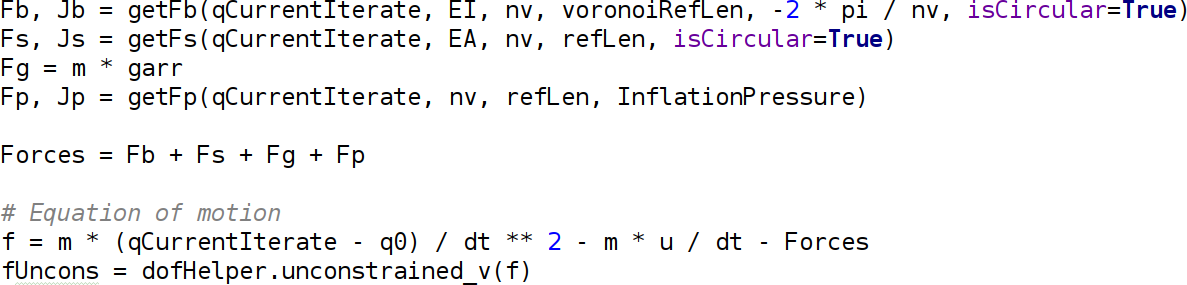
\includegraphics[width=\textwidth]{res/force.png}
		\end{center}
	\end{frame}
	\begin{frame}{What we did - Surface contact}
		In each frame:
		
		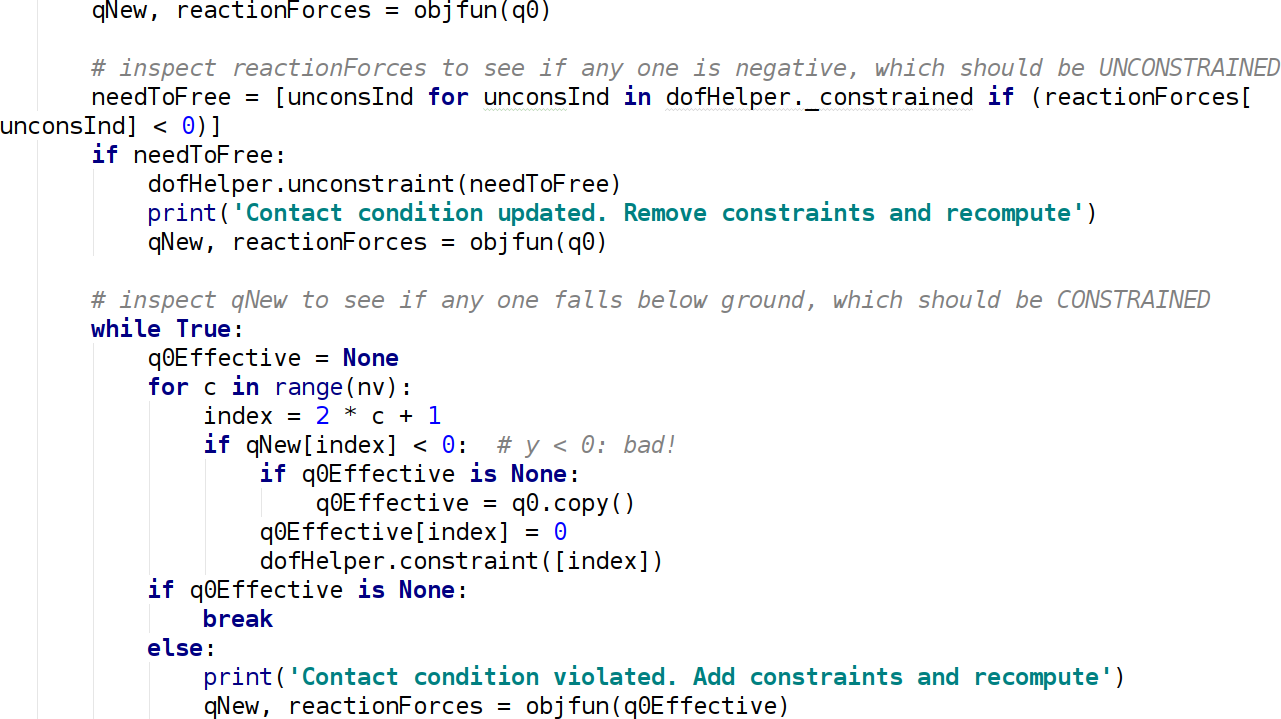
\includegraphics[width=1\textwidth]{res/corrector.png}
	\end{frame}
	\begin{frame}{All set!}
		\begin{tabular}{cc}
			Low pressure & High pressure\\
			\movie[width=4.615cm,height=4.665cm,showcontrols,poster,loop]{(Video: l-pressure)}{res/l-pressure.mp4} & 
			\movie[width=4.615cm,height=4.665cm,showcontrols,poster,loop]{(Video: h-pressure)}{res/h-pressure.mp4}
		\end{tabular}
	\end{frame}
	\begin{frame}{Project on GitHub now!}
		All code, results (and these slides) uploaded to
		
		\begin{center}
			\url{https://github.com/kmxz/mae259b-project}
			
			\qrcode[height=2.75cm]{https://github.com/kmxz/mae259b-project}
		\end{center}
	\end{frame}
\end{document}